\subsection{Funktionsprinzip}
\label{sub:funktionsprinzip}
    Für einen Datenaustausch zwischen Server und Client, sind in der fertigen Webanwendung folgende API\footnotemark Endpunkte vorhanden. 

    \footnotetext{Application Programming Interface}

    \begin{itemize}
      \item \textbf{/daily} stellt die Daten für das Zeitstrahldiagramm bereit und wird beim Start der Anwendung einmalig angefragt. Die Antwort enthält XY-Wertpaare. X stellt dabei die Zeit in Sekunden und Y die zu diesem Zeitwert aktiv werdenden Trips dar.

  \begin{lstlisting}[captionpos=t, caption=Antwort des Servers zur Anfrage \texttt{/daily}, label=lst:daily_response]
  [
    {"x":86340,"y":"6"},
    {"x":86400,"y":"10"}, 
    ...
  ]
  \end{lstlisting}

      \item \textbf{/trips/:from,:to} ermöglicht das Abfragen von Trips, die in einer Zeitspanne \texttt{from - to} aktiv sind. Beim initialen Aufruf der Webanwendung wird dieser Endpunkt als Erstes angefragt, um die aktiven Trips innerhalb einer Stunde zu erhalten. Der gewählte Zeitraum ist in Sekunden anzugeben. 

      Die Antwort des Servers auf einen Endpunkt vom Typ \texttt{/trips/} ist ein Objekt mit der Trip\_Id, dessen Inhalt der \texttt{GeoJSON} Spezifikation nach RFC 7946 folgt:

  \begin{lstlisting}[captionpos=t, caption=Trip Objekt, label=lst:trip_object]
  {
    2498: {  
      "type": "FeatureCollection",
      "features": [
        {
          "type": "Feature",
          "properties": {
            "name": "shape",
            ...
          },
          "geometry": {
            "type": "LineString",
            "coordinates": [[9.4437,48.64482], ...]
          }
        },
        {
          "type": "Feature",
          "properties": {
            "name": "station"
          },
          "geometry": {
            "type": "Point",
            "coordinates": [9.443688, 48.6448]
          }
        },
        ...
      ]
    }
  }
  \end{lstlisting}
    
      Da die Antwort in Listing \ref{lst:trip_object} mittels "`..."' gekürzt ist, sind detailliertere Antworten im \nameref{sec:anhang} unter Listing \ref{lst:geojson_featurecollection}, \ref{lst:shape_feature} und \ref{lst:station_feature} zu finden.

      \item \textbf{/trips/:id} antwortet mit den zur ID gehörenden Trip-Informationen. Dieser Endpunkt ermöglicht es, Informationen für nur einen einzigen Trip zu bekommen. Dies ist vor allem dann hilfreich, wenn der Nutzer ein Vehilce anklickt und Informationen über diesen Trip angezeigt bekommen möchte. Beispiel: \texttt{/trips/51295}

      \item \textbf{/trips/new/:from,:to,:tripIds} stellt die Abfrage für neue Trips zur Verfügung und exkludiert dabei diejenigen Trips, die in \texttt{:tripIds} genannt sind. Damit wird verhindert, dass bereits auf der Karte vorhandene Trips nicht doppelt auftauchen können. Dieser Query wird in einem 30 Sekunden-Intervall vom Client an den Server gesendet, um die neusten Trips zu erhalten. Damit wird die Karte aktuell gehalten. Beispiel: Es ist 10:00 Uhr, hole die in der nächsten Minute aktiv werdenden Trips (Zeitraum 10:00 bis 10:01 Uhr) und schließe die Trips mit der ID \texttt{51295,9212,52} vom Ergebnis aus \texttt{/trips/new/36000,36060,51295,9212,52}.

      \item \textbf{/trips/new/:from,:to} stellt die gleiche Funktionalität wie der vorherige Endpunkt zur Verfügung, mit der Ausnahme, dass keine Trip-ID's übermittelt werden müssen. Dieser Endpunkt ist beispielsweise dafür da, falls die Karte leer ist und noch keine aktiven Trips enthält.

    \end{itemize}

  % subsubsection api_endpunkte (end)

  Das generelle Prinzip der Webanwendung beruht auf einer Client / Server Architektur. Der Nodejs Server stellt verschiedene Endpunkte mittels Express als ansprechbare Routen dem Client zur Verfügung. 

  \begin{figure}[htbp]
    \begin{center}
      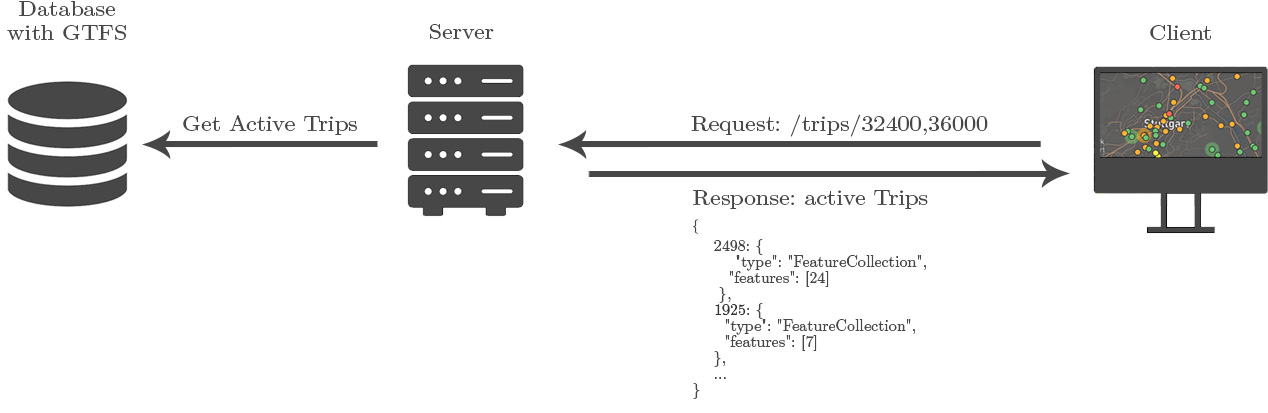
\includegraphics[width=\textwidth]{server_client.jpg}
      \caption{Server / Client Relation}
      \label{fig:server_client}
    \end{center}
  \end{figure}

  Trifft eine valide Anfrage auf den \texttt{/trips/:from,:to} Endpunkt, so wird ein Ablauf nach Abbildung \ref{fig:server_client} angestoßen.
  Die eintreffenden Anfragen werden vom Server entgegengenommen, validiert, verarbeitet und anschließend die entsprechende Antwort zurückgesendet. Die Validierung prüft die vom Client übergebenen Parameter auf ihre Plausibilität. Schlägt diese Prüfung fehl, wird ein Fehler vom Server zurückgegeben und der Server wartet auf eine neue Anfrage. Die wichtigste Routine des Servers stellt die Abfrage von Trips aus der Datenbank dar. Die Datenbank sucht diejenigen Trips heraus, welche in dem benötigten Zeitraum \texttt{from, to} aktiv sind. Dabei wird das Datum und der Wochentag zum Zeitpunkt der Anfrage verwendet. Um die Rechenarbeit im Client zu minimieren, werden alle Daten bei denen dies möglich ist, auf dem Server vorberechnet. Die aus der Datenbank abgefragten Daten durchlaufen folgenden Transformationsprozess:

  \begin{itemize}
    \item \textbf{Daten Mapping:} Die Trips aus der Datenbank werden in das \texttt{GeoJSON}-Format umgewandelt, damit diese im weiteren Programmverlauf einfacher zu verarbeiten sind. Dabei werden die im Kapitel "`\ref{sub:begriffe} \nameref{sub:begriffe}"' festgelegten Regeln beachtet.

    \item \textbf{Zurückgelegte Distanz:} Damit eine Animation der Vehicle stattfinden kann, ist die Berechnung der Distanzen zwischen den einzelnen Stationen nötig. 

    Falls das Feld dist\_traveled\footnotemark in der Datenbank vorhanden ist, kann die zurückgelegte Distanz sehr einfach daraus berechnet werden. Ist dies nicht der Fall so wird das in Abschnitt \ref{ssub:station_matching} beschriebene Station Matching durchgeführt, um die Distanzen berechnen zu können.
    \footnotetext{Die zurückgelegte Distanz bis zu einer Station $S$}

    \item \textbf{Feststellen der Richtung:} Für eine Polyline ist es unerheblich, ob die Koordinaten in der Reihenfolge $\{ p_1, p_2, \dotsc, p_n \}$ oder $\{ p_n, \dotsc, p_2, p_1 \}$ angeordnet sind. Damit das Vehicle aber in die richtige Richtung von $A$ nach $B$ fährt, ist es wichtig, dass die Koordinaten der Polyline in aufsteigender Reihenfolge festgelegt werden. Falls dies nicht er Fall ist, werden die Koordinaten in ihrer Reihenfolge umgekehrt.

    \item \textbf{Zeit zwischen Stationen:} In diesem Schritt wird die Fahrzeit (in sec) zwischen den einzelnen Stationen der Trips vorberechnet.

    \item \textbf{Codieren der Polyline:} Hier werden die Koordinaten in einen Polyline-String codiert.

    \item \textbf{Versenden:} Zuletzt wird die Anfrage des Clients vom Server mit einem Response-Paket beantwortet und der Prozess ist damit abgeschlossen bis eine neue Anfrage den Server erreicht.
  \end{itemize}
    
% subsection funktionsprinzip (end)